\documentclass{article}
\usepackage{arxiv}

\usepackage[utf8]{inputenc}
\usepackage[english, russian]{babel}
\usepackage[T1]{fontenc}
\usepackage{url}
\usepackage{booktabs}
\usepackage{amsfonts}
\usepackage{nicefrac}
\usepackage{microtype}
\usepackage{lipsum}
\usepackage{graphicx}
\usepackage{svg}
\usepackage{natbib}
\usepackage{doi}
\usepackage{booktabs}



\title{Классификация дуктов для поиска ключевых слов в рукописном контексте}

\author{ Феоктистов Дмитрий Дмитриевич \\
	ВМК МГУ\\
	\texttt{feoktistovdd@my.msu.ru} \\
	%% examples of more authors
	\And
	Местецкий Леонид Моисеевич \\
	ВМК МГУ\\
	\texttt{mestlm@yandex.ru} \\
}
\date{2023}

\renewcommand{\shorttitle}{Классификация дуктов для поиска ключевых слов в рукописном контексте}

%%% Add PDF metadata to help others organize their library
%%% Once the PDF is generated, you can check the metadata with
%%% $ pdfinfo template.pdf
\hypersetup{
pdftitle={Поиск ключевых слов в рукописном контексте},
pdfsubject={q-bio.NC, q-bio.QM},
pdfauthor={Феоктистов Д.Д., Местецкий Л.М.},
pdfkeywords={First keyword, Second keyword, More},
}

\begin{document}
\maketitle
\begin{abstract}
	В работе решается задача поиска ключевых слов в рукописном контексте. Пусть даны изображения некоторого рукописного файла, в котором требуется находить все вхождения введенного слова. Решение этой задачи может значительно упростить работу с архивными данными. Для решения задачи предлагается работать со словами на уровне их штрихового представления и определить метрику на множестве штрихов, с помощью которой можно решить задачу их классификации. Данный классификатор предлагается использовать как часть ранжирующего алгоритма. Для демонстрации результатов работы используются изображения работ участников ''Тотального диктанта''.
 % После чего строится алгоритм ранжирования слов, использующий информацию о классах штрихов запроса и слов контекста. Для демонстрации результатов работы используются изображения работ участников ''Тотального диктанта''.
\end{abstract}


\keywords{Обнаружение ключевых слов \and Преобразование Фурье \and Обучение метрик \and Компьютерное зрение}

\section{Введение}
\par Задача поиска ключевых слов в рукописном контексте является актуальной последние десятилетия в силу того, что полноценное распознавание рукописного текста не достигло той точности, при которой можно выполнять полноценное чтение документа и поиск в нем \citep{10.1007/978-3-031-36616-1_15, SOUIBGUI202243}. Одной из главной целей при решении задачи является достижение ее применимости для навигации в архивных документах \citep{10.1007/978-3-319-13695-0_74, 7333824}. 
\par Изначально задача поиска ключевых слов решалась для напечатанных документов, в которых используется курсивный шрифт \citep{627095}. Постепенно задача стала усложняться, и появились алгоритмы, выполняющие поиск в рукописных текстах \citep{1211511}, .
\par Существует несколько разновидностей рассматриваемой задачи. В первом варианте запрос задается в виде примера искомого слова в данном документе, такой подход позволяет обойти проблему разнообразия почерков \citep{7333824, 8378004}. Более общий подход предполагает, что запрос является строкой \citep{retsinas2021from}. Путей решения задачи также существует несколько. Первый предполагает использование глубоких нейронных сетей напрямую \citep{10.1007/978-3-031-41676-7_26, 10.1007/978-3-031-06555-2_26, Cascianelli2022}, второй -- использование нейронных сетей для построения векторных представлений слов для осуществления последующего поиска \citep{retsinas2021from, Krishnan2023, jemni2023stkeys}. Третий же стоит отдельно и предполагает использование признаков, полученных из изображения с помощью некоторых алгоритмов, с последующим их применением в алгоритмах машинного обучения. При этом может использоваться как и дискретное представление слов \citep{8270021, yousfi2021keyword, kundu2021hough}, так и непрерывные признаки, полученные из скелетных графов \citep{7333824, ameri2017keyword, stauffer2016graph}. Последний подход является актуальным и по сей день \citep{yousfi2021keyword, kundu2021hough, banerjee2022z}, так как есть экспериментально подтвержденная гипотеза о том, что увеличение количества параметров в нейронных сетях не приводит к улучшению результатов поиска \citep{rusakov2018expolring}. Наиболее актуальные алгоритмы используют комбинацию описанных подходов, применяя как и классические признаки, так и полученные с помощью обучения нейронной сети \citep{jemni2023stkeys, omayio2023word}.
\par Отдельно стоит выделить алгоритмы, выполняющие сопоставление запроса и слова с помощью различных метрик. Этот подход интересен тем, что метрики являются интерпретируемыми \citep{ameri2017keyword, stauffer2016graph}. При этом большинство метрик вычисляются долго, из-за чего требуется разработка специальных фильтров, позволяющих ускорять поиск \citep{stauffer2020filters}.
\par В данной работе предлагается новый метод решения задачи поиска ключевых слов в рукописном контексте, основанный на следующей гипотезе: все почерки являются вариацией некоторого эталонного. Действительно, уже несколько веков обучение письму производится с помощью прописей, в которых не меняются правила написания штрихов (дуктов), из которых строятся буквы. Соответственно, если задать метрику близости на штрихах и произвести их классификацию, то получится обоснованное представление слова в виде частично упорядоченного множества (порядок возникает из-за порядка появления штрихов). Имея описанное выше представление, можно производить поиск ключевых слов с помощью различных мер схожести множеств штрихов. Также описанная выше гипотеза позволяет решать задачу поиска ключевых слов в формулировке, в которой запрос передается в виде строки, которая преобразуется в изображение, написанное с помощью эталонного почерка (в данной работе с помощью шрифта Propisi). Насколько авторам известно, в подобной формулировке задача решалась в \citep{pronina2023frechet, pazazia2023dtw}, где для сравнения штрихов использовалось расстояние Фреше и DTW соответственно, но в этих работах рассматривался подход основанный на кластеризации, в то время как классификация способна дать больше информации. Таким образов в данной статье описаны:
\begin{enumerate}
\item Алгоритм выделения штрихов из изображения рукописного слова, основанный на построении скелета изображения.
\item Обучение метрики для задачи классификации на пространстве дуктов, основанной на преобразовании Фурье ломанных, описывающих штрихи.
% \item Мера сходства слов, использующая для поиска релевантных слов, основанная на расстоянии Левенштейна между множествами классифицированных дуктов.
\end{enumerate}
Для демонстрации результатов работы полученного алгоритма используются изображения работ участников ''Тотального диктанта''. Эти данные позволяют показать работоспособность подхода для различных почерков.
\section{Задача поиска ключевых слов в рукописном контексте}
Цель поиска ключевых слов состоит в том, чтобы извлечь изображения слов из заданной коллекции изображений документов и ранжировать их по релевантности определенному запросу. Запрос может быть либо уже найденным пользователем изображением слова (т.е. обрезанное изображение документа) (QbE), либо строкой, отвечающей слову, которое необходимо найти (QbS). Главным преимуществом второй постановки является отсутствие необходимости искать пользователю запрашиваемое слово самостоятельно, что сильно экономит время при работе с редкими словами, поэтому в данной работе рассматривается вариант QbS. Формализуем данную постановку. Пусть у нас есть множество строк $S$ и множество изображений слов $W$. Пусть $c(w)$ - строка, соответствующая изображению $w$. Тогда нам надо найти такое отображение $f: S \times W \rightarrow \mathbb{R}$, что:
$$argmin_w f(c(w_1), w) = w_1\;\;\;\forall w_1 \in W$$
В задаче поиска ключевых слов общепринятой метрикой является  $mean\; average\; precision$:
$$MAP = \frac{1}{|Q|}\sum_{q \in Q}AP(q)$$
Где $AP(q)$ -- площадь под кривой $precision-recall$ кривой для запроса $q$.\\
\section{Задача метрической классификации штрихов}
Математической моделью штриха является ломаная, которая может быть как замкнута, так и являться цепью. Существенным ограничением является отсутствие самопересечений у ломанных. Для сравнения штрихов предлагается ввести метрику, которую можно использовать в алгоритме классификации с помощью $k$ ближайших соседей. В качестве метрики задачи используется $accuracy$.
\section{Вычислительный эксперимент}
В качестве базового эксперимента предлагается решить задачу шестиклассовой классификации $1200$ сгенерированных штрихов. Каждый экземпляр датасета представляет собой искажение одного из типов ломанной, которая потенциально может встречаться в виде штриха Подробно описывать процесс генерации не буду, так как 27.10.2023 в 11:00 планируется утвердить классы и начать разметку данных, поэтому к middle talk здесь будет описание реальных данных, а выполнять одну и ту же работу дважды не хочется. Пример данных изображен на Рис. \ref{img:data_example}.\\
\begin{figure}
\centering
    \includesvg[width=0.4\linewidth]{syntetic_data.svg}
    \caption{Примеры сгенерированных данных, каждый объект является представителем своего класса.}
    \label{img:data_example}
\end{figure}
Будем сравнивать метрики, предложенные в \citep{pronina2023frechet, pazazia2023dtw}: расстояние Фреше между ломанными, DTW расстояние на коэффициентах сплайнов, аппроксимирующих ломанную, двумерное DTW расстояние между ломанными. Во всех трех случаях возьмем предобработку штрихов, которую использовали авторы. Расстояния будем сравнивать с помощью алгоритма $KNN$, как с равномерными весами, так и с весами, зависящими от расстояния. В качестве метрики воспользуемся средним значением $accuracy$ на кросс-валидации на пяти фолдах. Результаты эксперимента представлены на Рис. \ref{img:base_results}. Исходя из графика, можно сделать несколько выводов:
\begin{enumerate}
    \item Многомерное расстояние DTW является лучшим для классификации штрихов.
    \item Стоит брать количество соседей около $5$, так как с увеличением их количества точность не увеличивается, но может уменьшиться устойчивость алгоритма.
    \item Разницы между взвешенным и невзвешенным вариантами $KNN$ в рассматриваемой задаче нет.
\end{enumerate}
\begin{figure}
\centering
    \includesvg[width=0.6\linewidth]{preliminary_experiment.svg}
    \caption{Зависимость $accuracy$ на кросс-валидации от количества соседей в алгоритме $KNN$, синим отмечены значения для двумерного DTW, фиолетовым для расстояния Фреше, красным -- для DTW на коэффициентах сплайнов. Пунктиром отмечены запуски, при которых предсказания зависели от расстояний до соседей, а не только от их классов.}
    \label{img:base_results}
\end{figure}
% Традиционно в данной задаче используются метрики, используемые в информационном поиске. Пусть $w^i_s$ - изображение, стоящее на позиции $i$ в отсортированном по возрастанию значения $f(w, s)$ множестве $W$. Тогда определим метрики качества как:
% $$MAP@K = \frac{1}{|Q|}\sum_{q \in S}\frac{1}{K}\sum_{i=1}^K $$





% \section{Headings: first level}
% \label{sec:headings}

% \lipsum[4] See Section \ref{sec:headings}.

% \subsection{Headings: second level}
% \lipsum[5]
% \begin{equation}
% 	\xi _{ij}(t)=P(x_{t}=i,x_{t+1}=j|y,v,w;\theta)= {\frac {\alpha _{i}(t)a^{w_t}_{ij}\beta _{j}(t+1)b^{v_{t+1}}_{j}(y_{t+1})}{\sum _{i=1}^{N} \sum _{j=1}^{N} \alpha _{i}(t)a^{w_t}_{ij}\beta _{j}(t+1)b^{v_{t+1}}_{j}(y_{t+1})}}
% \end{equation}

% \subsubsection{Headings: third level}
% \lipsum[6]

% \paragraph{Paragraph}
% \lipsum[7]



% \section{Examples of citations, figures, tables, references}
% \label{sec:others}

% \subsection{Citations}
% Citations use \verb+natbib+. The documentation may be found at
% \begin{center}
% 	\url{http://mirrors.ctan.org/macros/latex/contrib/natbib/natnotes.pdf}
% \end{center}

% Here is an example usage of the two main commands (\verb+citet+ and \verb+citep+): Some people thought a thing \citep{kour2014real, hadash2018estimate} but other people thought something else \citep{kour2014fast}. Many people have speculated that if we knew exactly why \citet{kour2014fast} thought this\dots

% \subsection{Figures}
% \lipsum[10]
% See Figure \ref{fig:fig1}. Here is how you add footnotes. \footnote{Sample of the first footnote.}
% \lipsum[11]

% \begin{figure}
% 	\centering
% 	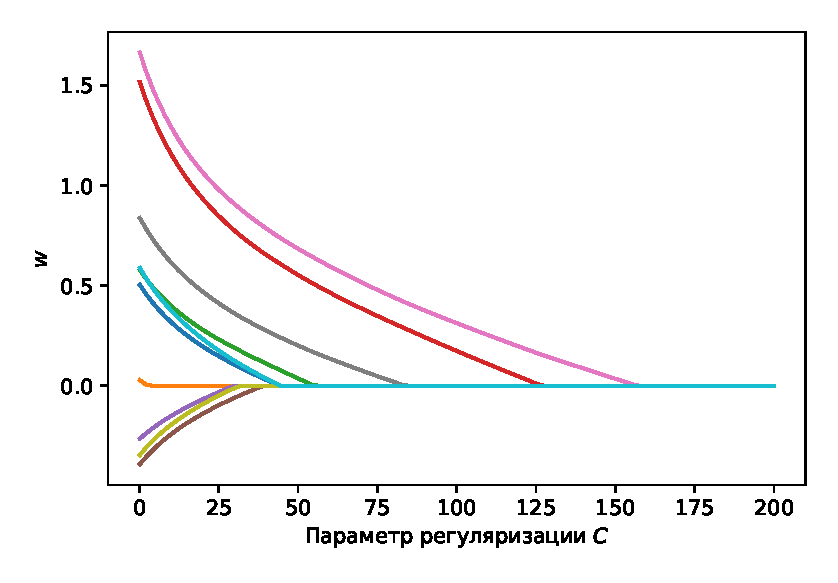
\includegraphics[width=0.5\textwidth]{../figures/log_reg_cs_exp.eps}
% 	\caption{Sample figure caption.}
% 	\label{fig:fig1}
% \end{figure}

% \subsection{Tables}
% See awesome Table~\ref{tab:table}.

% The documentation for \verb+booktabs+ (`Publication quality tables in LaTeX') is available from:
% \begin{center}
% 	\url{https://www.ctan.org/pkg/booktabs}
% \end{center}


% \begin{table}
% 	\caption{Sample table title}
% 	\centering
% 	\begin{tabular}{lll}
% 		\toprule
% 		\multicolumn{2}{c}{Part}                   \\
% 		\cmidrule(r){1-2}
% 		Name     & Description     & Size ($\mu$m) \\
% 		\midrule
% 		Dendrite & Input terminal  & $\sim$100     \\
% 		Axon     & Output terminal & $\sim$10      \\
% 		Soma     & Cell body       & up to $10^6$  \\
% 		\bottomrule
% 	\end{tabular}
% 	\label{tab:table}
% \end{table}

% \subsection{Lists}
% \begin{itemize}
% 	\item Lorem ipsum dolor sit amet
% 	\item consectetur adipiscing elit.
% 	\item Aliquam dignissim blandit est, in dictum tortor gravida eget. In ac rutrum magna.
% \end{itemize}


\bibliographystyle{unsrtnat}
\bibliography{references}

\end{document}